\documentclass[a4paper,10pt,oneside]{scrreprt}
\usepackage[latin1]{inputenc}
\usepackage[english]{babel}
\usepackage{graphicx}
\usepackage{float}
\usepackage{geometry}
\geometry{verbose,a4paper,tmargin=15mm,bmargin=25mm,lmargin=15mm,rmargin=15mm}
\usepackage{paralist}

\usepackage{paracol}

\usepackage{todonotes}

\usepackage{listings}
\lstset{language=Java,
	tabsize=2,
	showspaces=false,
	showtabs=false,
	breaklines=true,
	showstringspaces=false,
	breakatwhitespace=true,
	commentstyle=\color{pgreen},
	keywordstyle=\color{pblue},
	stringstyle=\color{pred},
	basicstyle=\footnotesize\ttfamily,
	moredelim=[il][\textcolor{pgrey}]{$$},
	moredelim=[is][\textcolor{pgrey}]{\%\%}{\%\%}
}

\usepackage{tikz}
\usetikzlibrary{calc,patterns,angles,quotes}

\usepackage{caption}
\usepackage{subcaption}
\usepackage{tabularx} % in the preamble

\usepackage{pdfpages}

%\usepackage{indentfirst} % for always indenting the first paragraphs

\usepackage{wrapfig}
\usepackage{lipsum}
\usepackage[linewidth=1.2pt,linecolor=red]{mdframed} % for boxes around wrapfigure and text

\begin{document}


\begin{center}
	Submitted by Group 18

	\bigskip

	\begin{tabular}{c}
	Group Members: \\
	CETIN, Ulfet (391819); GRUCZKA, FILIP (413279);	LIPINSKI, Bartosz (413177) \\
	SZYMANSKI, Bartosz (411949); GONG, Zeheng (378125)\\
	\end{tabular}

	\bigskip

	DIS1 WS 19/20 - Project Milestone II\\
	Ideation - Phase I\\

	%	(ordered on lastname basis)
\end{center}
\vspace{-1cm}

\begingroup
\let\clearpage\relax
	\chapter{The Problem \#1: Shopping for Kitchen}
\endgroup
				\vspace{-0.5cm}
				\textbf{Problem Statement:} People spending too much time deciding on what to buy for their refrigerators \& what to cook using the ingredients in the said refrigerator. Moreover, they get frustrated or bored because they spend so much time \& got a little gain from their spent time and effort.\\

				\vspace{2cm}
				\begin{center}
					\centering
					(go to the next page for the solutions)
				\end{center}


	\clearpage

	\section{Possible Six Solutions}

		\subsection{Solution \#1}

			\textbf{Definition:}\\
			\indent Informative screen in supermarkets that can be used for searching items with certain ingredients.\\

			\noindent \textbf{Use Case:}\\
			\indent The persona \textit{Helga Ratt} has a condition preventing her from eating gluten, and she cannot easily eat out as cheap places do not offer information about all the contents of a food, so she has to buy her products. If she wants to try something new that she did not eat before, she has to check the ingredients and read all the notifications on a packaging in order to see whether she can consume; and she dreads this as she lusts for some products but the time required is comparably abysmal to the pleasure of that food would bring.\\

			Market Helper! comes into play here. She can search for `Pizza` which contains `NO` amount of `gluten`, and Market Helper! would inform her about the whereabouts of the products that fits the criteria, saving Frau Ratt time. The screens can be installed to the supermarkets in couples, as each user would assumably take 5 minutes on the screen at most.\\

			The fun side of the MarketHelper! is that, via an optional VR glass, while traversing to grab the one pizza she wants to buy, she can smash other options of the said product(pizza) via a virtual mace in augmented reality, and she would be points that can be spent on the same brand of the pizza next time she wents shopping.

			\noindent \textbf{Storyboard:}\\

			\begin{figure}[H]
				\centering

				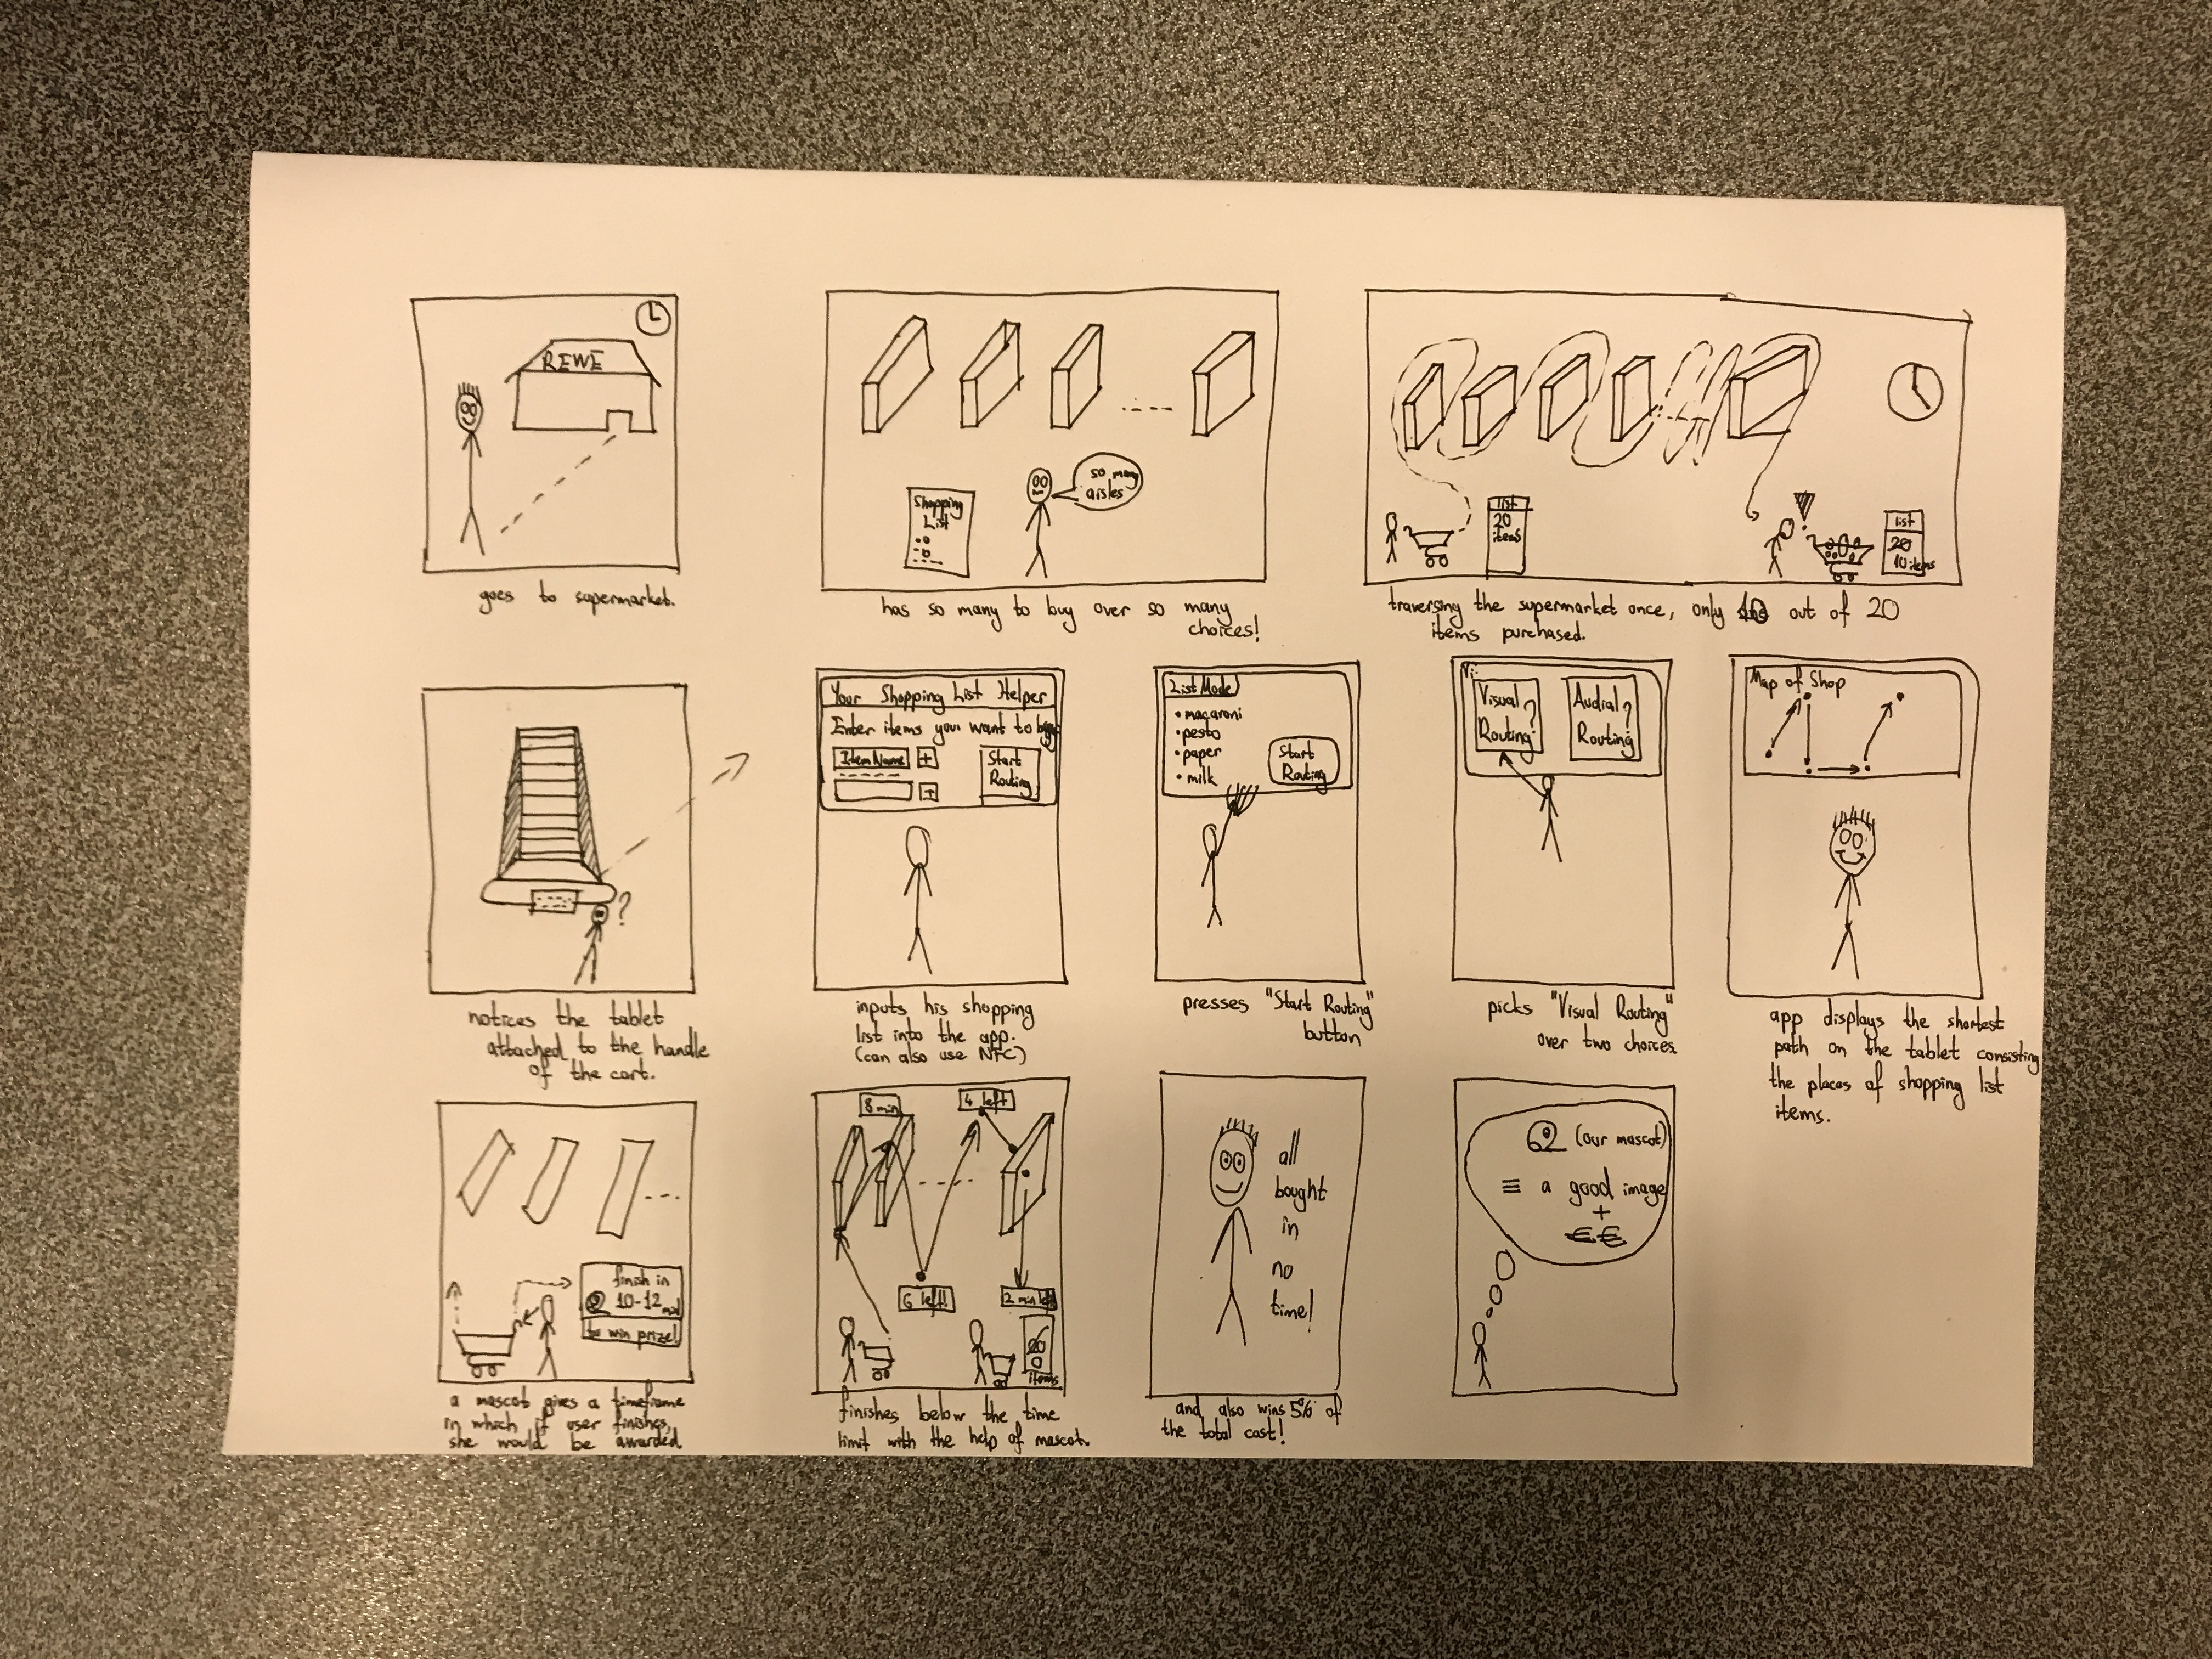
\includegraphics[scale=0.16, clip, trim={30em 0em 65em 10em}]{images/s2.jpg}
			\end{figure}

		\clearpage
		\subsection{Solution \#2}

			\noindent \textbf{Definition:}\\
			shopping assistants for supermarkets, which is placed on the handle of a shopping cart in the form of a smart tablet\\

			\noindent \textbf{Use Case:}\\
			Fulfilling a complete shopping list takes time, especially if users are not so aware of the layout a specific supermarket and whereabouts of the products that are needed. Asking to the employees not always help, as they are not always around or they just verbally inform once.\\

			Shopping List Helper! comes into play here. One can create a shopping list on the said tablet on the spot, or one can synchronize their shopping list at their phone via NFC. Then, SLH would lead the user via the shortest path either using a map of the supermarket together with the marker for the user, or via audial cues that are continuously feeded to the headphones of the user.\\

			The fun side of Shopping List Helper! is that the tablet screen involves a mascot that provides a countdown to the user, in the form of a time range (e.g. 10 minutes - 12 minutes) based on the products and the shortest path. If user manages to finish putting all the desired products in the cart and finally make the purchase, the user would be awarded with a small percentage of his purchase.

			\noindent \textbf{Storyboard:}\\

			\begin{figure}[h]
				\centering
				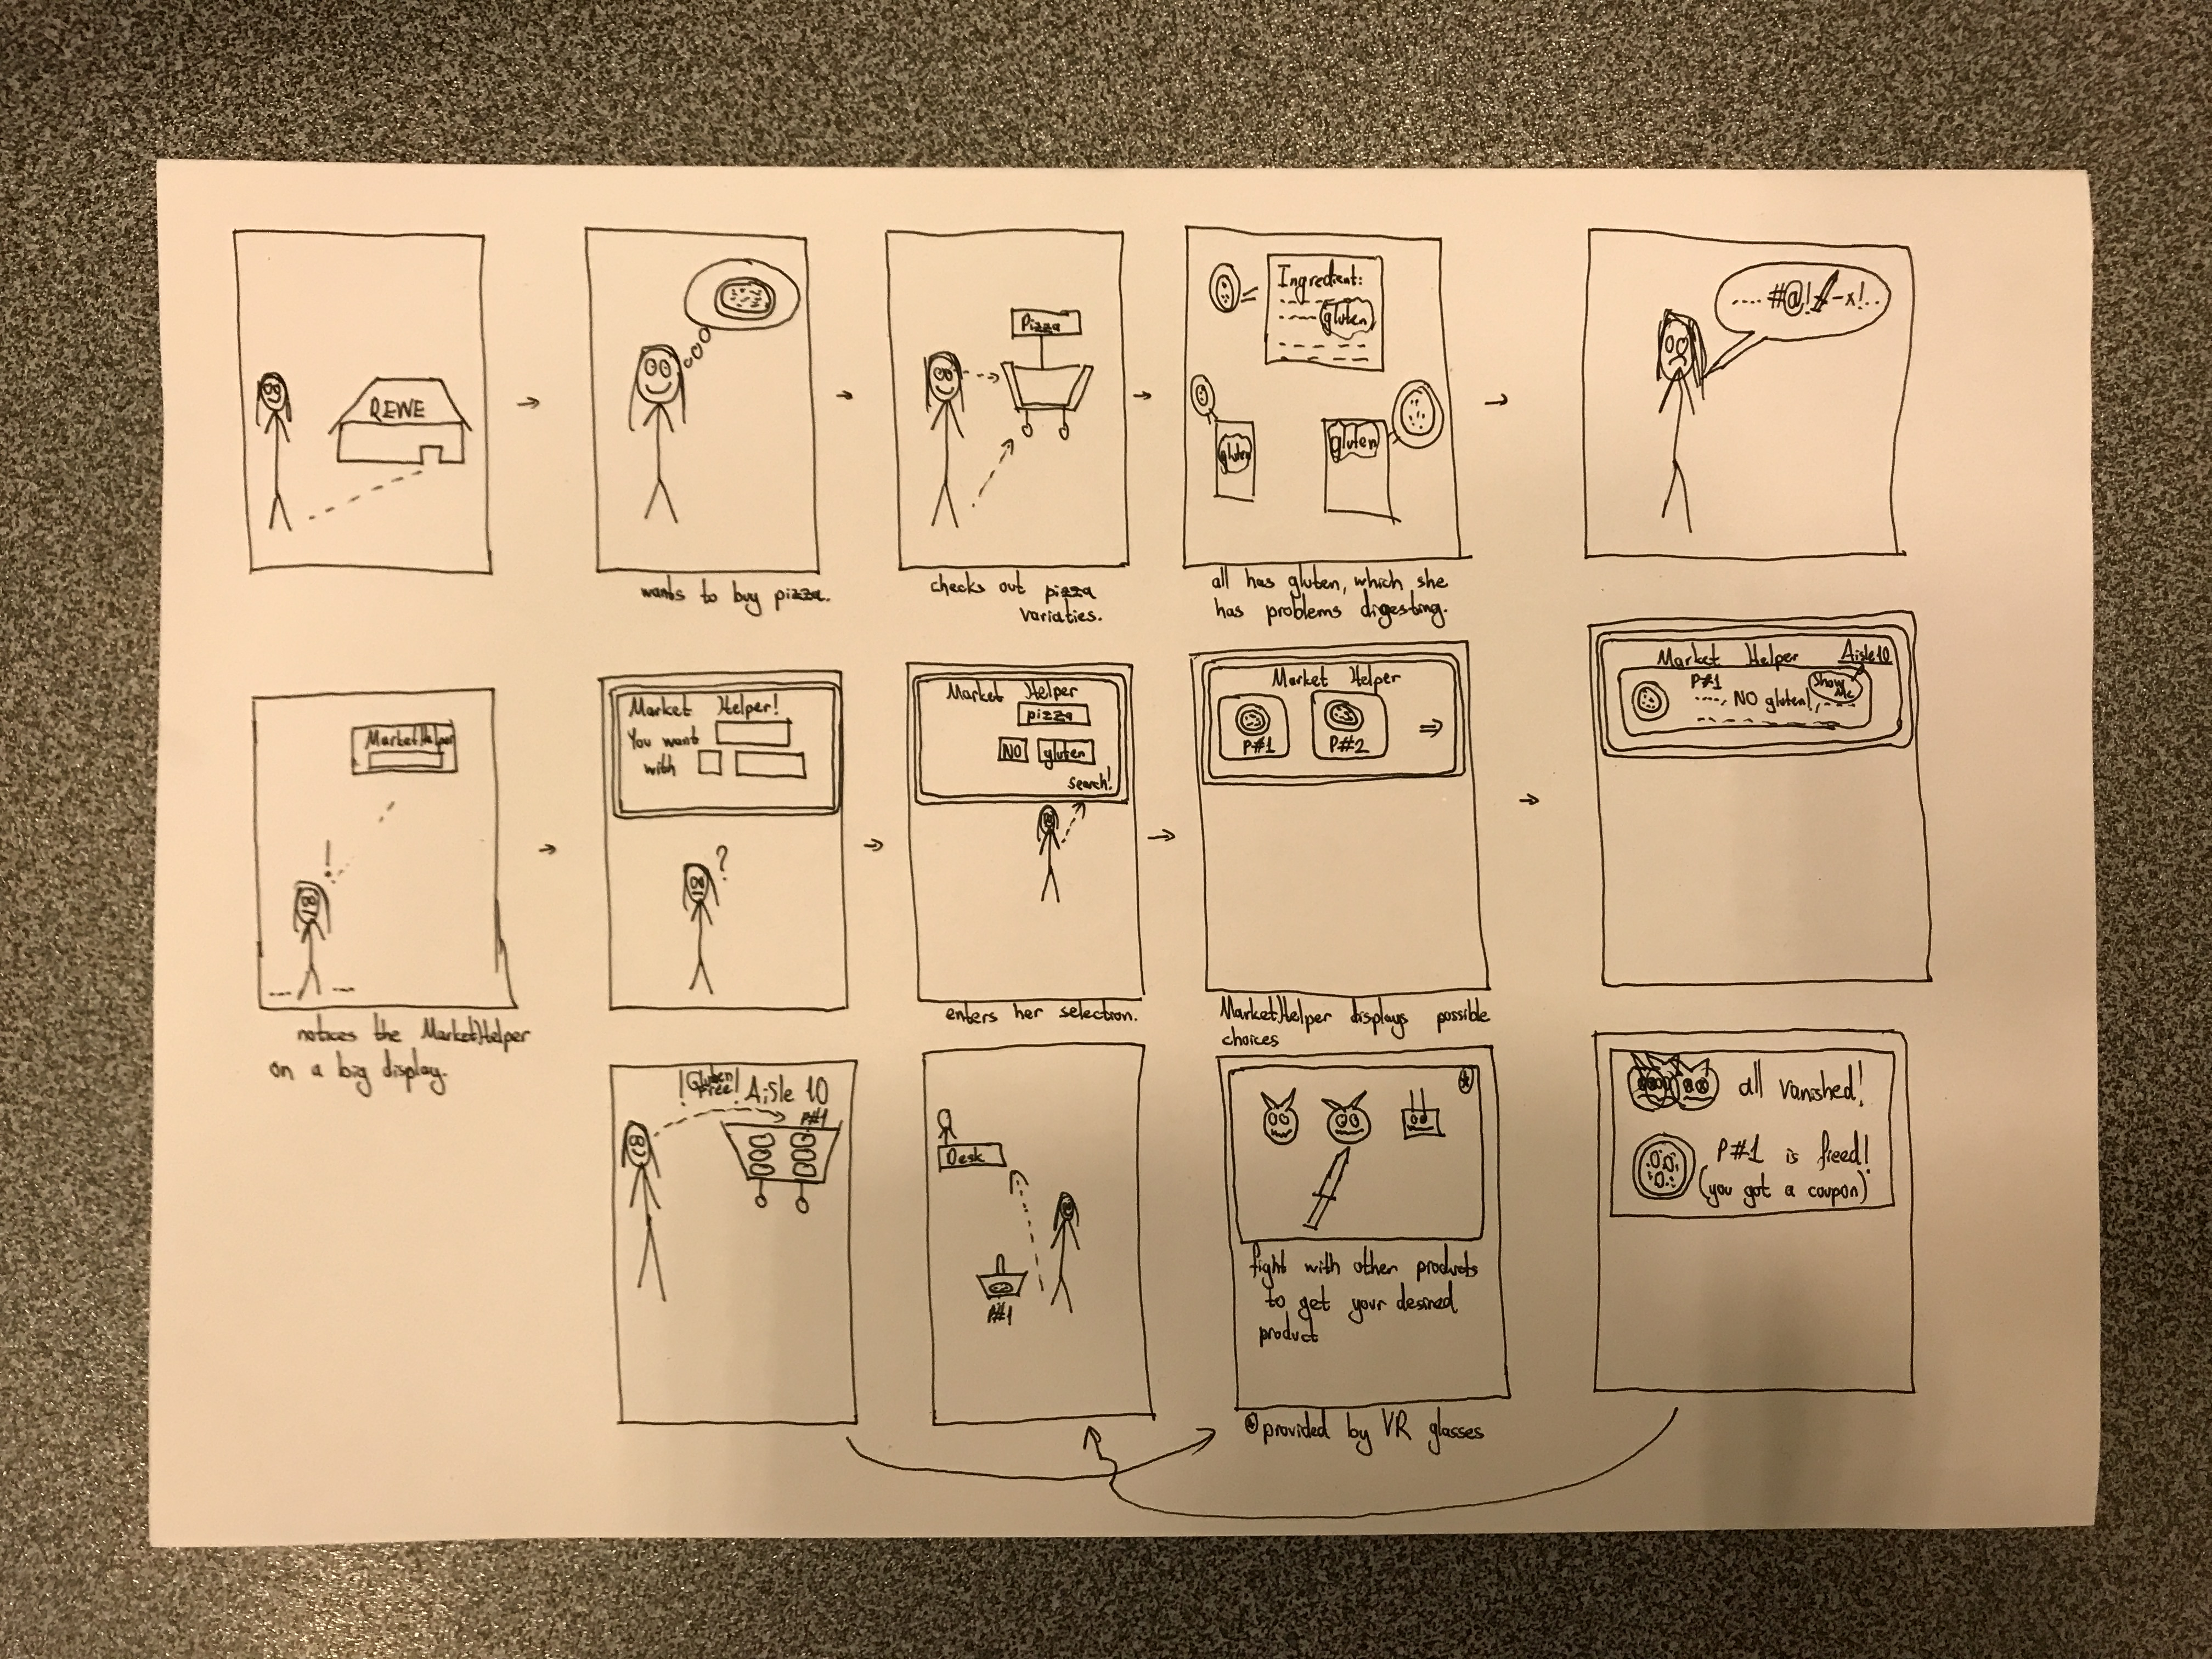
\includegraphics[scale=0.16, clip, trim={45em 0em 45em 0em}]{images/s1.jpg}
			\end{figure}

		\clearpage

		\subsection{Solution \#3}

		\noindent \textbf{Definition:}\\
			Meals presentation in supermarkets - user can try dish and after deciding on specific meal can take a bag with all ingredients needed to prepare the dish and go straight to the cash.\\

			\noindent \textbf{Use Case:}\\
			The persona "Mother" always would like to preper healthy food for her kids. She can't imagine buying fast food or
already prepared dishes (put to microwave for 3 min). Once she enter to the supermarket, with our solution she will
be able to get inspiration what to cook, she can try different dishes.\\

			Furthermore we will present massage chairs in which guests can seat. They will be resting and selecting preferred dish after work. We will present meals like in "sushi house" on the moving table. After decision what to cook, they doesn't have to
even look for ingredients, they can just take bag with all needs for specific meal and go straight to cash register.\\

			\noindent \textbf{Storyboard:}\\

			\begin{figure}[H]
				\centering
				\includegraphics[width=11cm]{example-image}
			\end{figure}

		\subsection{Solution \#4}

		\noindent \textbf{Definition:}\\
			System for learning kids about food and healthy eating. Tablet display on refrigerator, that shows what ingredients you have in the kitchen. Like self-service checkout in the market with animations for kids. You can simply increase number ingredient or decrease. Then once you are in supermarket, you can get notification what ingredians you have in the kitchen.\\

			\noindent \textbf{Use Case:}\\
			The persona "Mother" always go with kids to the supermarket on Saturdays and  Sundays. She always struggle to calm down her kids in the store, and she can't focus on shopping list. With our system kids can help her do shopping faster and in more funny way. Once the family is in the store the they will get notification about ingredients in the kitchen and what's missing. Then kids can take phone. By learning and watching cartoons provided by app, thay can help their mother to finish shopping quicker.\\

			The app basically will show needed ingredients and will learn kids about healthy eating. After come back to house, kids will help to sort products in the refrigerator.\\

			\noindent \textbf{Storyboard:}\\

			\begin{figure}[H]
				\centering
				\includegraphics[width=11cm]{example-image}
			\end{figure}

			\clearpage
			\subsection{Solution \#5}

				\noindent \textbf{Definition:}\\
				An enjoyable interactive system of groceries shopping in supermarkets for a balanced diet. The system uses barcode recognition to detect whether the groceries in the shopping cart are in a correct(balanced-diet) combination, i.e.: one serving of meat + one serving of vegetables + one serving of staple food. The display that combines with the shopping cart shows the total price of the groceries in the cart, therefore the user can control the budget. If there is a correct combination, the user got one reward point in her/his customer card after checking out. Users can redeem cash against the reward points.\\

				\noindent \textbf{Use Case:}\\
				As an undergraduate student of RWTH David is always stressful, not only about the study but also about life. On one side he does not have much time to shop groceries and prepare meals, on the other side he still wants to keep a balanced diet and hold the budget.\\
				\\
				With our system, David would get a real-time instruction about balance-diet and he can get reward from it at the same time. This system helps people forming a healthy habit and holding a budget. Simultaneously, this system makes the shopping experience more fun.\\

				\noindent \textbf{Storyboard:}\\

				\begin{figure}[h]
					\centering
					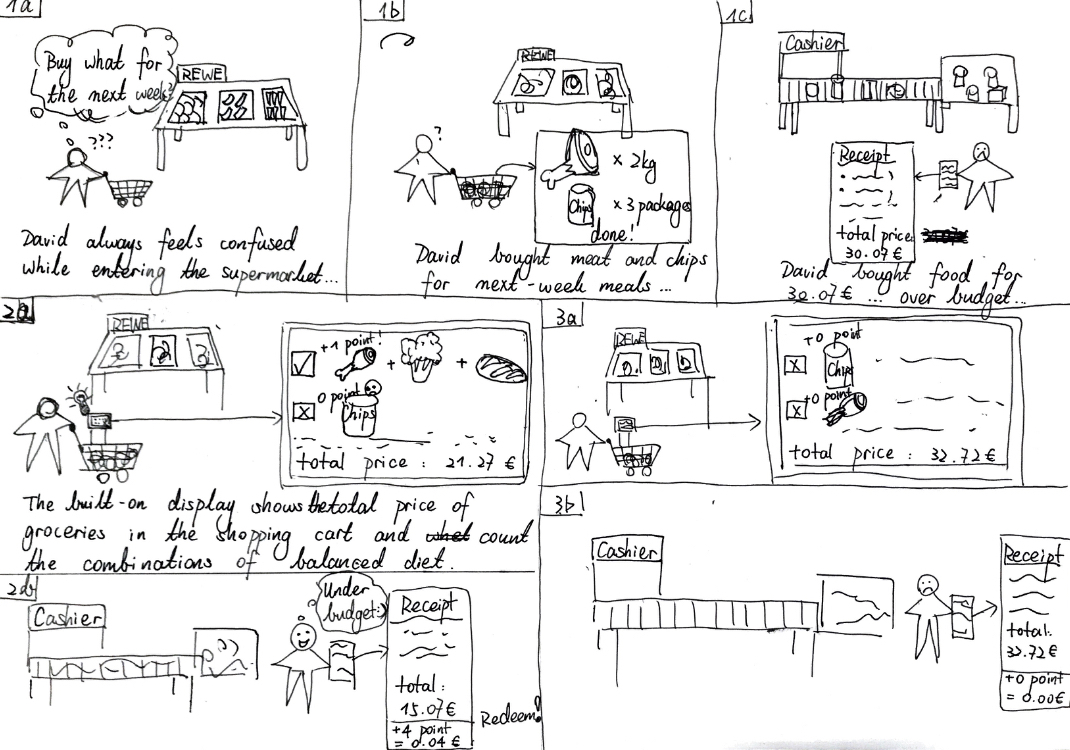
\includegraphics[scale=0.4, clip, trim={0em 0em 0em 0em}]{images/s5.jpg}
				\end{figure}

			\clearpage

		\bigskip

	\section{Six Storyboards}
		does not have to be in this order

	\section{Concept Map, Brainstorming Notes, Votes}
		have to include all the solutions

			\noindent \textbf{Concept Map:}\\

			\begin{figure}[H]
				\centering
				\includegraphics[width=11cm]{example-image}
			\end{figure}


	\section{Personas}

		\subsection{Persona \#1: Picky Eater Helga}

		Our extreme persona

		\begin{mdframed}
			\begin{minipage}{\textwidth}
				\begin{wrapfigure}{r}{0.2\textwidth}
					\centering
					\fbox{
\includegraphics[clip, trim=2cm 1cm 3cm 0cm, scale=0.63]{images/picky.jpg}}
					\vspace{-4cm}
				\end{wrapfigure}


				\textbf{Demographics:}\\
				35, female, single\\
				of Swedish and Canadian origin from the parents\\
				has M.Sc. in Gender Studies\\
				works in a Social Services in leading position, 40 hours/week\\
				novice user of technology\\
				has a condition which prohibits her from eating certain foods\\

				\textbf{Background:}\\
				Helga grew up in a poor household, and suffered the lack of money during her childhood. This led her to pick her profession where she can provide a helping hand to people in need. Outside her work, she spends her time reading books about mythology, and watching documentaries on various topics. She is an avid exerciser, and at her worst, she would go for a brisk walk for 2 hours.\\



%				\textbf{Motivation:}\\
%				working for the benefit of the World, and aiming to distribute the wealth of the World as equally as possible to people in need\\

%				spending less time cooking food
%				eating healthy
%				not wasting food\\


				\textbf{Frustrations:}
				not spending her time qualitatively\\
				not having trips abroad to observe other cultures\\
				having to keep working in a job that is taxing soul-wise
%				always eating the same things over and over
%				making foods go to waste
%				taking so much time thinking what groceries to buy
%				limited options for her health condition	\\


%				Meet \textbf{Helga Ratt}!\\
%
%				Entertains herself reading articles on healthy food and what food has which effect on the body and the mood of a person.\\
%
%
%
%				Oftenly, her health condition prevents her from eating out, and she has to look at the packaging of novel products in order to check whether they are safe for her to eat.\\
%
%
%
%				Although her friends call her `health nut` once in a while, she has a good physique and healthy body, and in addition to careful meal planning, she works out to keep herself top of her game.\\

%				She dreads spending so much time on shopping for food, as she sees shoppings as adventures first to discover new products that she can consume, then always come home with the same old tofu and like.\\
			\end{minipage}
		\end{mdframed}

		\subsection{Persona \#2: Mother}

		\textbf{Demographics:}\\
				Sarah Johnson\\
				female\\
				age: 40\\
				graduated university in Germany\\
				married\\
				mother of three kids\\
				work from 9am to 5pm\\
				living with husband and kids in rented house\\
				annual household income: 50 000 euro\\

		\textbf{Background:}\\
				Sarah was born and grown in Germany. She was living with parents in small countryside in the middle Germany. She he moved out from parents house when she was 18. Then Sarah moved to Frankfurt, where she started studing. She met there her current husband. After graduation, while looking for the jobs they moved to Aachen.\\

		\textbf{Behavior:}\\
				Sarah is very busy housewife and mother\\
				she love spend time with her husband and kids at home\\
				once a year she's going for holidays with her family\\
				she always forget things to do after, 8 hours of work. She doesn't like buying grocery products\\

		\textbf{Frustrations:}\\
				She is frustrated when she has to stay after hours at work. Sarah prefer to have less stressful work, even when earning less\\

		\textbf{Goals:}\\
				Sarah would like to spent as much time with her kids and husband at home\\


				\subsection{Persona \#3: David}
			\begin{mdframed}
				\begin{minipage}{\textwidth}
				\begin{wrapfigure}{r}{0.2\textwidth}
						\centering
						\fbox{
\includegraphics[clip, trim=0cm 0cm 0cm 0cm, scale=0.7]{images/David.jpg}}
						\vspace{-4cm}
					\end{wrapfigure}


					\textbf{Background:}\\
					20, male\\
	                undergraduate student of RWTH\\
	                studies Machine Engineering
	                single\\
	                heavy study workload(40+hours per week)\\



					\textbf{Motivation:}\\
					travel and experience other cultures\\
	                healthy lifestyle(both regular daily routine and diet)\\
	                coffee lover\\
	                play video games\\
	                hang out with a small group of friends at quiet coffee shops\\


					\textbf{Frustrations:}\\
					going out to bars at night\\
	                not enough free time for gaming\\
	                looks and fashion\\
	                \\
	                David loves technical things. He is an advanced user of mobile and desktop devices and social media. He goes to supermarket once a week because as a student at RWTH university he does not hat much time. But he still takes short trips at some weekends.\\
	                \\
	                \textbf{Quote from David:}\\
				''I wish I can combine work and travel in the future!''\\
				\end{minipage}
				\end{mdframed}


\end{document}}
